\let\cleardoublepage\clearpage
\section{Tableau des livrables}

\vspace{-1cm}
\begin{figure}[H]
\noindent\makebox[\textwidth]{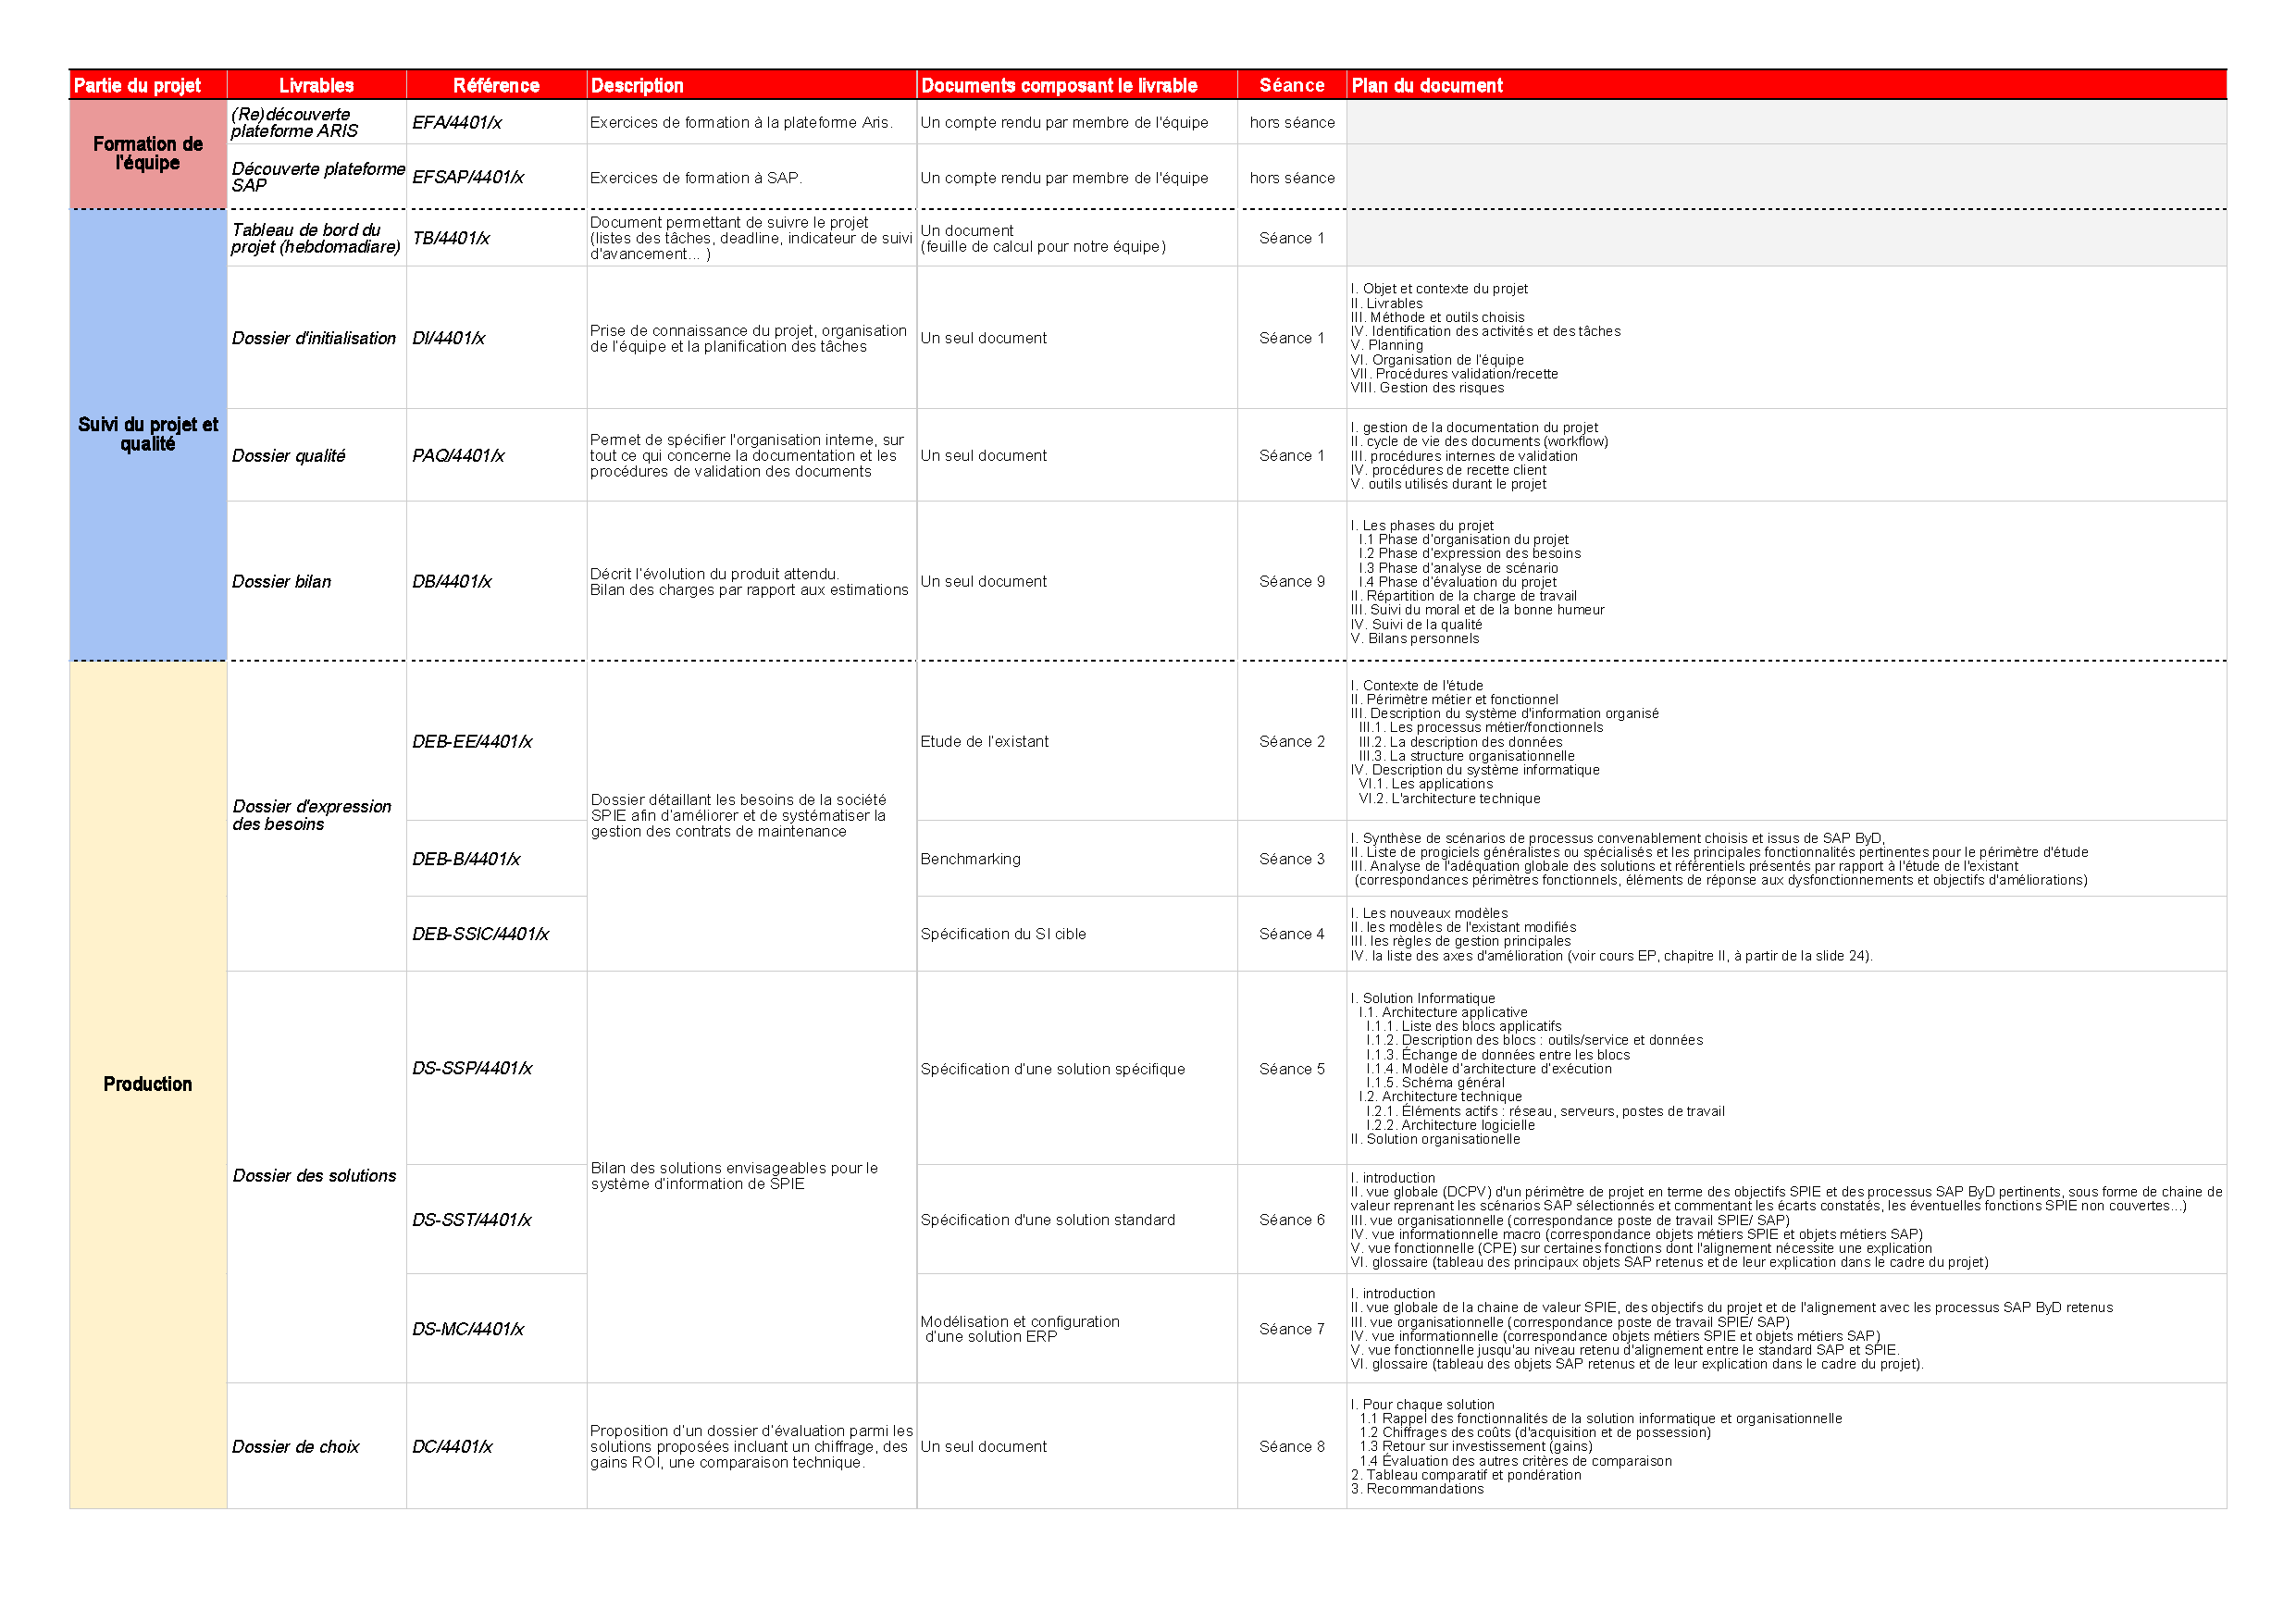
\includegraphics[width=20cm]{figures/livrables.pdf}}
\vspace{-3cm}
\caption{Tableau récapitulatif des livrables}
\end{figure}

\section{Description des documents attendus par phase du projet}

Cette partie permet de récapituler l’ensemble des livrables à remettre lors de chaque phase du projet, en présentant de manière synthétique leurs contenus. \\

Pour les plans de chaque document, il est nécessaire de se référer au tableau récapitulatif de chaque livrable.

\subsection{Phase d’initialisation}

\subsubsection{Le dossier d’initialisation}

Il s’agit du présent document. Son objectif est de décrire le but du projet, ainsi que son contexte en terme d’objectifs, de périmètre, d’acteurs. On y trouve également la description ci-présente des livrables. Le mode opératoire et les outils choisis y sont également définis.  \\

Ce document permet également l’identification des différentes activités et tâches, de façon à élaborer un planning du projet. \\

Enfin, il contient tous les éléments concernant notre équipe, tant en terme d’organisation qu’en terme de gestion des risques.

\subsubsection{Le PAQ}

Le PAQ ou Plan d’Assurance Qualité permet de décrire la façon dont notre équipe s’organise pour produire les livrables attendus avec la meilleure qualité qui soit. \\

Ainsi, on retrouve tout ce qui concerne la gestion de la documentation du projet et le cycle de vie des documents produits. Notre processus de validation interne est documenté, de même que les procédures de recette client. \\

Enfin, il liste l’ensemble des outils utilisés durant le projet et explicite le rôle de chacun de ces derniers dans le projet, c’est-à-dire l’exploitation que l’équipe fera de ces outils.

\subsubsection{Tableau de bord du projet (hebdomadiare)}

Une description avec des captures d’écran du tableau de bord permettant le suivi de projet sera remise avec le dossier d’initialisation. Le tableau de bord doit à tout instant donner une image fiable de l’avancement du projet et doit permettre de suivre ce dernier de manière fine afin de détecter toute irrégularité tel qu’un glissement au niveau du planning ou une chute du moral global de l’équipe.

\subsection{Phase de formation}

\subsubsection{(Re)Découverte de la plateforme ARIS}

Chaque membre de l’équipe doit rendre un compte rendu de 2 pages sur son ressenti lors de l’initiation qui consiste en la réalisation d’un exercice ARIS simple.

\subsubsection{Découverte plateforme SAP}

Chaque membre de l’équipe doit rendre un compte rendu de 2 pages sur son ressenti lors de l’initiation.

\subsection{Phase d’expression des besoins}

\subsubsection{Étude de l'existant}

Le but de ce rapport est de documenter l’organisation existante au sein de SPIE selon trois grands axes, qui sont l’axe fonctionnel, l’axe organisationnel et l’axe informatique, afin d’en établir les avantages et les inconvénients.\newline
Le rapport doit comporter environ une dizaine de pages.

\subsubsection{Benchmark}

Ce livrable peut s'appuyer sur des modèles ARIS. Ce rapport intermédiaire doit comprendre : \\

\begin{description}
    \item[\textbullet] Un résumé des scenarii des processus correctement élu depuis SAP ByD.
    \item[\textbullet] Un listing de progiciels avec des fonctionnalités intéressantes dans le cadre de l’étude.
    \item[\textbullet] Vérification de la conformité des solutions développées par rapport à l’existant.
\end{description}

\subsubsection{Spécification du SI cible}

Il s’agit ici de fournir un rapport intermédiaire concernant la modélisation en utilisant le formalisme ARIS. Ce rapport contiendra notamment : \\
\begin{description}
    \item[\textbullet] Les nouveaux modèles,
    \item[\textbullet] les modèles de l'existant modifiés,
    \item[\textbullet] les règles de gestion principales,
    \item[\textbullet] et la liste des axes d'amélioration.
\end{description}

\subsection{Phase : Dossier des solutions}

\subsubsection{Spécification d’une solution spécifique}

Les spécifications se présenteront sous la forme d’un rapport qui documente les dimensions fonctionnelle, organisationnelle et informatique de la solution.

\subsubsection{Spécification d’une solution standard}

La spécification de la solution standard comprend : \\
\begin{description}
    \item[\textbullet] La description de la solution standard à l’aide de modèle correspond aux besoins de SPIE, incluant le référentiel SAP ByD de manière à voir les enjeux organisationnels
    \item[\textbullet] L’ensemble des scénarii SAP sélectionnés
    \item[\textbullet] Enfin, il contiendra :
        \begin{description}
            \item[\textbullet] les matrices ARIS montrant l’accord entre les processus élaborées par notre équipe et ceux de SPIE,
            \item[\textbullet] les fonctions SAP,
            \item[\textbullet] et l’organigramme de SPIE.
        \end{description}
\end{description}

\subsubsection{Modélisation et configuration de la solution ERP}

Il s’agit à nouveau d’un rapport généré par ARIS qui contiendra : \\

\begin{description}
    \item[\textbullet] Les modèles permettant de décrire la solution standard répondant aux besoins de SPIE avec le standard SAP ByD, a un niveau suffisant pour permettre le dimensionnement du projet, 
    \item[\textbullet] la configuration des scénarii SAP sélectionnés,
    \item[\textbullet] et des matrices ARIS montrant l’accord entre les processus élaborés par notre équipe, et ceux de SPIE.
\end{description}

\subsection{Phase : Bilan}

\subsubsection{Évaluation des solutions}

Il s’agit ici de remettre \bf{un dossier de choix}. Celui doit mettre en avant les forces et faiblesses de chaque solution proposée par notre équipe.

\subsubsection{Restitution}

La restitution finale est constitué de deux livrables. On trouve : \\

\begin{description}
    \item[\textbullet] Une présentation
    \item[\textbullet] Un dossier bilan \\
\end{description}

Ces deux livrables auront pour but de donner l’ensemble des éléments quantitatifs concernant le projet, de manière à détailler les compétences acquises sous la forme d’un tableau.
